\documentclass[letterpaper,  %a4paper
               %boxit,
               %titlepage,   % separate title page
               %refpage      % separate references
              ]{jacow-2_3}   %jacow}
%
% CHANGE SEQUENCE OF GRAPHICS EXTENSION TO BE EMBEDDED
% ----------------------------------------------------
% test for XeTeX where the sequence is by default eps-> pdf, jpg, png, pdf, ...
%    and the JACoW template provides JACpic2v3.eps and JACpic2v3.jpg which
%    might generates errors, therefore PNG and JPG first
%
\makeatletter%
	\ifboolexpr{bool{xetex}}
	 {\renewcommand{\Gin@extensions}{.pdf,%
	                    .png,.jpg,.bmp,.pict,.tif,.psd,.mac,.sga,.tga,.gif,%
	                    .eps,.ps,%
	                    }}{}
\makeatother

% CHECK FOR XeTeX/LuaTeX BEFORE DEFINING AN INPUT ENCODING
% --------------------------------------------------------
%   utf8  is default for XeTeX/LuaTeX 
%   utf8  in LaTeX only realizes a small portion of codes
%
\ifboolexpr{bool{xetex} or bool{luatex}} % test for XeTeX/LuaTeX
 {}                                      % input encoding is utf8 by default
 {\usepackage[utf8]{inputenc}}           % switch to utf8

\usepackage[USenglish]{babel}			 

\usepackage[final]{pdfpages}
\usepackage{multirow}
\usepackage{ragged2e}
\usepackage{tikz}
\usetikzlibrary{shapes,arrows,snakes,backgrounds}
\usetikzlibrary{mindmap,trees}
\usetikzlibrary{decorations.pathreplacing}
\usetikzlibrary{plotmarks}
%
% if BibLaTeX is used
%
\ifboolexpr{bool{jacowbiblatex}}%
 {%
  \addbibresource{jacow-test.bib}
  \addbibresource{biblatex-examples.bib}
 }{}
\listfiles

%
% command for typesetting a \section like word
%
\newcommand\SEC[1]{\textbf{\uppercase{#1}}}

%%
%%   Lengths for the spaces in the title
%%   \setlength\titleblockstartskip{..}  %before title, default 3pt
%%   \setlength\titleblockmiddleskip{..} %between title + author, default 1em
%%   \setlength\titleblockendskip{..}    %afterauthor, default 1em

%\copyrightspace %default 1cm. arbitrary size with e.g. \copyrightspace[2cm]

% testing to fill the copyright space
%\usepackage{eso-pic}
%\AddToShipoutPictureFG*{\AtTextLowerLeft{\textcolor{red}{COPYRIGHTSPACE}}}

\begin{document}

\title{Bunch length measurements using CTR at the AWA with comparison to simulation}

\author{N. Neveu\thanks{nneveu@anl.gov}\textsuperscript{1}, 
	    L. Spentzouris, Illinois Institute of Technology, Chicago, USA \\
		A. Halavanau, P. Piot, Northern Illinois University, DeKalb, USA \\
	    J. G. Power, \textsuperscript{1}Argonne National Laboratory}
\maketitle

%
\begin{abstract}
In this paper we present electron bunch length measurements 
at the Argonne Wakefield Accelerator (AWA) photoinjector facility. 
The AWA accelerator has a large dynamic charge density range, 
with electron beam charge varying between 0.1 nC - 100 nC, 
and laser spot size diameter at the cathode between 0.1 mm - 18 mm. 
The bunch length measurements were taken at different charge densities 
using a metallic screen and a Martin-Puplett interferometer to perform 
autocorrelation scans of the corresponding coherent transition radiation (CTR). 
A liquid helium-cooled 4K bolometer was used to register the interferometer signal. 
The experimental results are compared with Impact-T and OPAL-T numerical simulations.
\end{abstract}


\section{AWA Facility}
The AWA Facility houses two rf photoinjectors, both 
operating at \SI{1.3}{GHz}. The photoinjector used for 
these studies consists of a gun and solenoids followed
by six accelerating cavities, as shown in Fig.~\ref{fig:beamline}. 
This beam line is capable of low (\SI{0.1}{nC}) and 
high charge (\SI{100}{nC}) operation. The bunch charge is 
routinely adjusted for depending on the requirements 
of the experiments downstream of the photoinjector.
Typical operating charges are 1, 4, 10, and \SI{40}{nC}. 
While these are the most
common operating modes, other charges have been requested 
and provided depending on the experiment.
Recent experiments include emittance exchange \cite{eex}, 
structure tests \cite{pets}, thermal emittance measurements \cite{therm}, 
and two beam acceleration \cite{tba}. 


\section{CTR Measurement Technique}
Describe what CTR is here

\section{Simulations}
Simulations of the AWA beam line shown in Fig~\ref{beamline}
were performed in the PIC codes IMPACT~\cite{impact} and OPAL~\cite{opal}.
The gun, accelerating cavities, and solenoids were modeled with 2D
Poisson Superfish~\cite{fish} files. All field maps were in the T7 format. 

\begin{figure*}[!tbh]
	\centering
	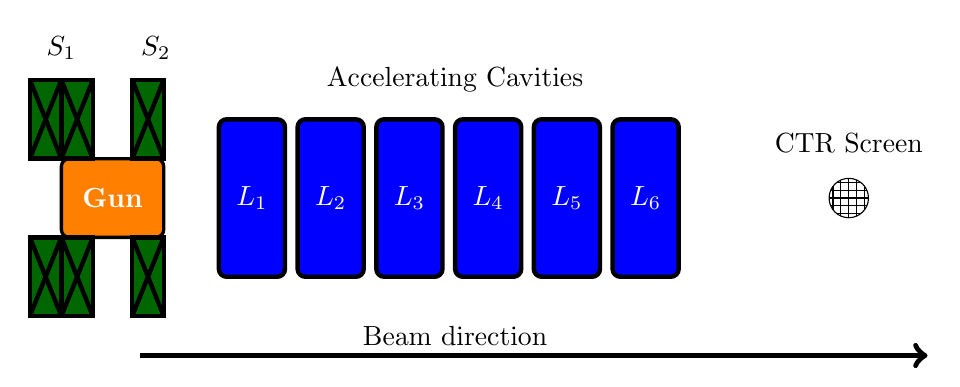
\begin{tikzpicture}[scale=1.0, text=black]
	\def \gunleft {-1.0}
\def \gunright {0.3}
\def \loneright {1.0}
\def \ltworight {2.0}
\def \lthreeright {3.0}
\def \lfourright {4.0}
\def \lfiveright {5.0}
\def \lsixright {6.0}
\def \quadone {7.5}

%Line between kicker and septum
\node[] at (4.0,-0.75) {Beam direction};
\draw[line width=0.75mm, ->] (0.0,-1.0) -- (10,-1.0);

\draw[fill=orange, very thick, rounded corners =0.1cm] (\gunleft,0.5)rectangle (\gunright,1.5) node[pos=.5, white] {\textbf{Gun}} ;
%S1
\node[] at (-1,2.9) {$S_1$};
\draw[ultra thick, fill=black!60!green] (-1.4,-0.5)rectangle  (-1.0,0.5) node[pos=.5, white] {} ;
\draw[black, ultra thick] (-1.4,-0.5) -- (-1.0,0.5);
\draw[black, ultra thick] (-1.4,0.5) -- (-1.0,-0.5);
\draw[ultra thick, fill=black!60!green] (-1.4,1.5)rectangle  (-1.0,2.5) node[pos=.5, white] {} ;
\draw[black, ultra thick] (-1.4,1.5) -- (-1.0,2.5);
\draw[black, ultra thick] (-1.4,2.5) -- (-1.0,1.5);
%S2
\draw[ultra thick, fill=black!60!green] (-1.0,-0.5)rectangle  (-0.6,0.5) node[pos=.5, white] {} ;
\draw[black, ultra thick] (-1.0,-0.5) -- (-0.6,0.5);
\draw[black, ultra thick] (-1.0,0.5) -- (-0.6,-0.5);
\draw[ultra thick, fill=black!60!green] (-1.0,1.5)rectangle  (-0.6,2.5) node[pos=.5, white] {} ;
\draw[black, ultra thick] (-1.0,1.5) -- (-0.6,2.5);
\draw[black, ultra thick] (-1.0,2.5) -- (-0.6,1.5);

%S3
\node[] at (0.2,2.9) {$S_2$};
\draw[ultra thick, fill=black!60!green] (-0.1,-0.5) rectangle  (0.3,0.5) node[pos=.5, white] {};
\draw[black, ultra thick] (-0.1,-0.5) -- (0.3,0.5);
\draw[black, ultra thick] (-0.1,0.5) -- (0.3,-0.5);
\draw[ultra thick, fill=black!60!green] (-0.1,1.5) rectangle  (0.3,2.5) node[pos=.5, white] {};
\draw[black, ultra thick] (-0.1,1.5) -- (0.3,2.5);
\draw[black, ultra thick] (-0.1,2.5) -- (0.3,1.5);
%Linac drawings 
\node[] at (4,2.5) {Accelerating Cavities};
\draw[fill=blue, ultra thick, rounded corners =0.1cm] (\loneright,0)rectangle  ({\loneright+0.84},2) node[pos=.5, white] {$L_1$} ;
\draw[fill=blue, ultra thick, rounded corners =0.1cm] (\ltworight,0)rectangle  ({\ltworight+0.84},2) node[pos=.5, white] {$L_2$};
\draw[fill=blue, ultra thick, rounded corners =0.1cm] (\lthreeright,0)rectangle ({\lthreeright+0.84},2) node[pos=.5, white] {$L_3$};
\draw[fill=blue, ultra thick, rounded corners =0.1cm] (\lfourright,0)rectangle ({\lfourright+0.84},2) node[pos=.5, white] {$L_4$};
\draw[fill=blue, ultra thick, rounded corners =0.1cm] (\lfiveright,0)rectangle ({\lfiveright+0.84},2) node[pos=.5, white] {$L_5$};
\draw[fill=blue, ultra thick, rounded corners =0.1cm] (\lsixright,0)rectangle ({\lsixright+0.84},2) node[pos=.5, white] {$L_6$};



%current optimization point
%\node[draw, fill=yellow, star, star points=5, star point ratio=0.6, minimum size=0.1cm]
%at (12.5,1.0) {$z_1$};
\node[] at (9,1.7) {CTR Screen};
\clip[draw] (9,1) circle (0.25cm);
\draw[step=1mm] (-1,-1) grid (10,10);



%\draw[latex-latex] (\gunleft,-5.0) -- (14,-5.0) ;
%\foreach \x in  {0.3, 1.0, 3.5, 5.0, 7.0, 8.5, 10, 12.5} %tick marks
%\draw[shift={(\x,-5.0)},color=black] (0pt,3pt) -- (0pt,-3pt);
%\foreach \x in {0.3, 1.0, 3.5, 5.0, 7.0, 8.5, 10, 12.5}
%\draw[shift={(\x,-5.2)},color=black] (0pt,0pt) node[below] {$\x$};

%Line between kicker and septum
\draw[very thick] (13.25,0.2) -- (14.5,-0.5);


%Line between septum and dipole
\draw[very thick] (15.6,-0.5) -- (16.5,-0.5);




	\end{tikzpicture}	
	\caption{Beam line layout at the AWA.}
	\label{beamline}
\end{figure*}

\begin{table}[hbt]
	%   \vspace*{-.5\baselineskip}
	\centering
	\caption{Simulation Parameters}
	\begin{tabular}{lcc}
		\toprule
		\textbf{Parameter} & \textbf{Low Charge}  & \textbf{High Charge} \\
		\midrule
		Charge       & \SI{1}{nC}        & \SI{40}{nC}    \\ %[3pt]
		Gun Gradient & \SI{65}{MV/m}     & \SI{65}{MV/m}  \\ %[3pt]
		$S_1$        & \SI{500}{A}		 & \SI{500}{A}	  \\
		$S_2$		 & \SI{}{A}   	 & \SI{185}{A}		 \\
		Linac Phases & On crest          & On crest       \\
		Laser FWHM   & \SI{1.5}{ps}      & \SI{1.5}{ps}   \\ %[3pt]
		Laser Radius & \SI{2}{mm}        & \SI{9}{mm}     \\
		\bottomrule
	\end{tabular}
	\label{simparam}
	%   \vspace*{-\baselineskip}
\end{table}


\section{Experimental Setup}
The beam line layout is shown in Fig.~\ref{fig:beamline}. 
Bunches were allowed to propagate freely to the 
CTR screen. The only focusing elements used were solenoids $S_1$ and
$S_2$. As the bunches passed the CTR screen, light was
emitted through a window located next to the screen, 
as shown in Fig.~\ref{inter}. A slit was used to prevent
background x-rays from reaching the bolometer.
After passing the slit, the light was captured 
using an interferometer outside the beam line, 
also shown in Fig~\ref{inter}. 
A remotely movable leg inside the interferometer was swept, 
and the resulting signal fed to the bolometer, 
which is shown in Fig.~\ref{bolo}. The bolometer 
was cooled with liquid helium. Period refilling of
the helium was required throughout the day in order
to keep the bolometer at \SI{4}{K}.
 
\begin{figure}
	\begin{tikzpicture}[every node/.style={anchor=south west,inner sep=0pt},x=1mm, y=1mm,]   
	\node (fig1) at (0,0)
	{\includegraphics[width=0.5\textwidth]{images/interferometer}};
	\node[fill=white, inner sep=2pt] (txt2) at (35,15) {Interferometer};
	\node[fill=white, inner sep=2pt, rotate=26] (txt2) at (18,19.5) {Slit};	
	\node[fill=white, inner sep=2pt, rotate=20] (txt2) at (13,27) {Window};
	\end{tikzpicture}
	\caption{Interferometer used to capture CTR light as it exited a 
			window on the beam line. }
	\label{inter}
\end{figure}

\begin{figure}
	\begin{tikzpicture}[every node/.style={anchor=south west,inner sep=0pt},x=1mm, y=1mm,]   
	\node (fig1) at (0,0)
	{\includegraphics[width=0.5\textwidth]{images/bolometer}};
	\node[fill=white, inner sep=2pt] (txt2) at (35,8) {Interferometer};	
	\node[fill=white, inner sep=2pt] (txt2) at (55,25) {Window};	
	\node[fill=white, inner sep=2pt] (txt2) at (22,35) {Bolometer};
	\end{tikzpicture}
	\caption{Bolometer. }
	\label{bolo}
\end{figure}








\section{Data Analysis}
Give link to code used to find bunch length

\section{Results}
Compare simulations to experimental measurements
\begin{figure}[!htb]
	%   \vspace*{-.5\baselineskip}
	\centering
	%\includegraphics*[width=174pt]{JACpic_mc}
	\caption{Layout of papers.}
	\label{l2ea4-f1}
	%   \vspace*{-\baselineskip}
\end{figure}

\section{Conclusion}
Any conclusions should be in a separate section directly preceding
the \SEC{Acknowledgment}, \SEC{Appendix}, or \SEC{References} sections, in that
order.

\section{acknowledgments}
We would like to thank 
Northern Illinois University (NIU) for providing the 
interferometer used in this experiment. 
We also gratefully acknowledge the computing resources
provided on Bebop, a high-performance computing cluster
operated by the LCRC at Argonne National Laboratory.
This material is based upon work supported by the 
U.S. Department of Energy, Office of Science, under 
contract number DE-AC02-06CH11357 and grant number DE-SC0015479. 
Travel to IPAC'18 supported by the Division of Physics 
of the United States National Science Foundation 
Accelerator Science Program and the Division of 
Beam Physics of the American Physical Society.


\begin{thebibliography}{9}
\bibitem{eex}
A.~Alpha and B.~T.~Beta, “EEX....”
in \textit{Proc. IPAC’17}, 
Copenhagen, Denmark, May 2016, 
paper xxx, pp. xxx--xxx.\\

\bibitem{pets}
A.~Alpha and B.~T.~Beta, “PETS....”
in \textit{Proc. IPAC’17}, 
Copenhagen, Denmark, May 2016, 
paper xxx, pp. xxx--xxx.\\

\bibitem{therm}
A.~Alpha \emph{et al.}, “THERM....”
in \textit{Proc. IPAC’17}, 
Copenhagen, Denmark, May 2016, 
paper xxx, pp. xxx--xxx.\\

\bibitem{tba}
A.~Alpha and B.~T.~Beta, “TBA....”
in \textit{Proc. IPAC’17}, 
Copenhagen, Denmark, May 2016, 
paper xxx, pp. xxx--xxx.\\

\bibitem{item:2-2}
A.~Alpha \emph{et al.}, 
“A fascinating paper about FELs,”
in \emph{Proc. FEL’13}, 
New York, NY, USA, Aug. 2013, 
paper WEP033, pp. 27--29.\\

\bibitem{impact}
J.~Qiang \emph{et al.},
“...,”
, California, USA,
Rep. xxxx, 20xx-20xx.

\bibitem{opal}
A.~Adelmann \emph{et al.},
“The OPAL (Object Oriented Parallel Accelerator Library) framework,”
PSI, Zurich, Switzerland,
Rep. PSI-PR-08-02, 2008-2017.

\end{thebibliography}


\section{jacow notes...}
Figure captions are placed below figures, and table
captions are placed above tables.

Figure captions are formatted as shown in Figs.~\ref{l2ea4-f1} and \ref{l2ea4-f2},
while table captions take the form of a heading,
with initial letters of principle words, capitalized, and
without a period at the end (see Tables~\ref{eq:units} and \ref{style-tab}).
Any reference to the contents of the table should be made from
the body of the paper rather than from within the table
caption itself.

 Single-line captions are centered in the column, while captions
that span more than one line should be justified.
The \LaTeX\ template uses the ‘booktabs’ package to
format tables.

If a displayed equation needs a number (i.\,e., it will be
referenced), place it it in parentheses, and flush with the
right margin of the column. The equation itself should be
indented and centered, as far as is possible:
\begin{equation}\label{eq:units}
    C_B=\frac{q^3}{3\epsilon_{0} mc}=\SI{3.54}{\micro eV/T}
\end{equation}

When referencing a numbered equation, the equation number is placed
in parentheses [e.g., Eq. (1)].

\section{checklist for electronic publication}

\begin{Itemize}
	\item  Use only Times or Times New Roman (standard, bold or italic) and Symbol
	fonts for text---\SI{10}{pt} minimum except references, which can be \SI{9}{pt} or \SI{10}{pt}.
	\item  Figures should use Times or Times New Roman (standard, bold or italic) and
	Symbol fonts when possible---\SI{6}{pt} minimum.
	\item  Check that citations to references appear in sequential order and
	that all references are cited.
	\item  Check that the PDF file prints correctly.
	\item  Check that there are no page numbers.
	\item  Check that the margins on the printed version are within \SI{\pm1}{mm}
	of the specifications.
	\item  \LaTeX\ users can check their margins by invoking the
	\texttt{boxit} option.
\end{Itemize}

\subsubsection{Author Listing} Careful attention should be given to the
placing of commas and the use of ‘and’ in the author list.
In particular, for the case of six or more authors
(Ref. [3]), a comma also follows the penultimate author.
The preference for ‘\emph{et al.}’\ takes precedence when the number
of authors becomes large (e.g., $>$6).

\subsection{Alignment of References}

In the \LaTeX\ template, \verb|\bibliography{9}| is used for
when the total number of references is less than ten. This
should be changed to \verb|\bibliography{99}| if the number of
references is ten or more.



\patchcmd\thebibliography{\section*{REFERENCES\@mkboth {REFERENCES}{REFERENCES}}}{}{}{}
\section{PAPER PUBLISHED IN A CONFERENCE PROCEEDINGS}

\definecolor{jgreen}{cmyk}{0.81, 0.00, 0.97, 0.00}
\definecolor{jred}{cmyk}  {0.00, 0.99, 1.00, 0.00}
\definecolor{jgrepc}{cmyk}{0.74, 0.05, 1.00, 0.00}
\definecolor{jblue}{cmyk} {0.87, 0.54, 0.00, 0.00}
\definecolor{jvio}{cmyk}  {0.41, 0.82, 0.00, 0.00}
\definecolor{jbook}{cmyk} {0.28, 0.88, 0.79, 0.25}
\definecolor{jrept}{cmyk} {0.07, 0.70, 1.00, 0.00}
\definecolor{jmanu}{cmyk} {0.28, 0.77, 1.00, 0.23}
\definecolor{junpu}{cmyk} {0.00, 0.83, 0.65, 0.00}


\section{PAPER PRESENTED AT THE CURRENT CONFERENCE}

\subsection{Abbreviated Form}

\begin{thebibliography}{9} % Use for 1-9 references
\setcounter{enumi}{4}
	\bibitem{item:52}
	A.~Alpha and B.~T.~Beta, 
	“An interesting talk,”
	presented at IPAC’16, 
	Busan, Korea, May 2016, 
	paper MOAB01, this conference.\\
	\textcolor{jgrepc}{[Current conference; conference name in normal font; the
		wording “this conference” is optional]}
\end{thebibliography}

\section{PAPER PUBLISHED IN, OR SUBMITTED TO, A PERIODICAL}
\begin{thebibliography}{99} % Use for 1-9 references
  \setcounter{enumi}{5}
	\bibitem{item:6}
		P.~Mercury \emph{et al.}, 
		“Title of paper published in journal,”
		\emph{Phy. Rev. Lett.}, vol. 114, no. 5, 
		p. 050511, Feb. 2014. \\
	\textcolor{jblue}{[Periodical, Phys. Rev. Lett.; 
		             issue no. and month may be omitted]}

	\bibitem{item:7}
		P.~Venus \emph{et al.}, 
		“New techniques in laser wakefield accelerators,”
		\emph{Phys. Rev. ST Accel. Beams}, vol. 18, 
		p. 120198, Dec.~2015.   \\
	\textcolor{jblue}{[Periodical, Phys. Rev. ST Accel. Beams; 
			              month may be omitted]}

	\bibitem{item:8}
		T.~Earth \emph{et al.}, 
		“Low dose irradiation impact on modern silicon detectors,”
		\emph{Nucl. Instr. Meth.}, vol. 692, pp. 256--280, 2014.
	\textcolor{jblue}{[Periodical, Nucl. Instr. Method.]}
	
	\bibitem{item:9}
		T.~Earth, L.~Moon, and A.~Belt, 
		“Temporal correlations of x-ray free electron lasers,”
		\emph{Optics Express}, vol. 20, pp. 11396--11404, 2012.
	\textcolor{jblue}{[Periodical, Optics Express]}

	\bibitem{item:10}
		J.~B.~Good, 
		“A paper accepted for publication,”
		\emph{Phys. Rev. Lett.}, to be published.
	\textcolor{jblue}{[Periodical, paper accepted for publication 
		              by Phys. Rev. Lett.]}

	\bibitem{item:11}
		G.~D.~Read, 
		“Title of paper submitted for publication,”
		submitted for publication.
	\textcolor{jblue}{[Paper submitted for publication; the name of the 
					  periodical does not appear]}
\end{thebibliography}

\section{ONLINE SOURCE}

\begin{thebibliography}{99} % Use for 1-9 references
  \setcounter{enumi}{11}
	\bibitem{item:121}
		JACoW, \url{http://www.jacow.org} \\
		\textcolor{jvio}{[online source; no hyperlink, no period at end of URL
						  unless there is a trailing “/” as shown below. A monospace
						  font, such as Lucida Sans Typewriter (size 8 pt), is used in
					      Word, while the ‘url’ package in \LaTeX\ uses the Latin Modern Typewriter font]}

\end{thebibliography}

\section{CITATIONS TO BOOKS}

\begin{thebibliography}{99} % Use for 1-9 references
	\setcounter{enumi}{12}
	\bibitem{item:13}
		T.~Earth and L.~Moon, 
		“Title of chapter in the book,”
		in \emph{Title of Book}, R Mars, Ed. New York, NY, USA: 
		Wiley, 1994, pp.~42--48. \\
	\textcolor{jbook}{[Chapter in book]}
	
	\bibitem{item:14}
		A.~Belt, \emph{Title of Book}. Cambridge, MA, USA: 
		MIT Press, 1986. \\
	\textcolor{jbook}{[Book]}
\end{thebibliography}

\section{REPORTS AND THESES}

\begin{thebibliography}{99} % Use for 1-9 references
	\setcounter{enumi}{14}
	\bibitem{item:15}
		G. Jupiter \emph{et al.}, 
		“Title of report,” CERN, Geneva, Switzerland,
		Rep. CERN-2012-333, Oct. 2012.\\
	\textcolor{jrept}{[Report]}

	\bibitem{item:16}
		A.~Student, “Title of thesis,”
		Ph.D. thesis, Phys. Dept.,
		Karlsruher Institut für Technologie, Karlsruhe, 
		Germany, 2014.\\
	\textcolor{jrept}{[Thesis]}
\end{thebibliography}


\section{MANUAL}

\begin{thebibliography}{99} % Use for 1-9 references
	\setcounter{enumi}{16}
	\bibitem{item:17}
		\emph{IEEE Editorial Style Manual}, 
		IEEE Periodicals, 
		Piscataway, NJ, USA, Oct. 2014, pp. 34-52; 
		\url{http://www.ieee.org/documents/style_manual.pdf} \\
	\textcolor{jmanu}{[Handbook/Manual, no hyperlink, no period after URL]}
\end{thebibliography}


\section{UNPUBLISHED WORK AND PRIVATE COMMUNICATION}

\begin{thebibliography}{99} % Use for 1-9 references
	\setcounter{enumi}{18}
	\bibitem{item:19}
		P.~Neptune, “Title of paper,” unpublished.\\
	\textcolor{junpu}{[Unpublished]}
	
	\bibitem{item:20}
	P.~Uranus, private communication, Jun. 2015.\\
	\textcolor{junpu}{[Private communication]}

\end{thebibliography}
\null  % this is a hack for correcting the wrong un-indent by package 'flushend' in versions before 2015

\subsection{Figure Captions}

Figure captions should be placed below the figure and
centered if on one line, but justified if spanning two or
more lines:
\begin{center}
	Figure 1: A one line figure caption is centered.
\end{center}
\begin{justify}
	Figure 2: A lengthy figure caption that spans 
	two lines is justified.
\end{justify}
Note the colon “:” after the figure number and the period
“.” at the end of the caption.

\subsection{Table Headings}

Table captions should be placed above the table and
centered if on one line, but justified if spanning two or
more lines:
\begin{center}
	Table 1: Table Heading
\end{center}
\begin{justify}
	Table 2: A Particularly Long Table Heading 
	Spanning Two Lines
\end{justify}

Note the colon ":" after the table number, that the initial
letters of the principle words in the table heading are
capitalized, and the absence of a period at the end of the
caption.


\subsection{Equations}

If a displayed equation requires a number, it should be
placed flush with the right margin of the column. Please
leave sufficient space immediately before and after the
equation,




\end{document}
	
